\documentclass{beamer}
\usetheme{Boadilla}

\usepackage[utf8]{inputenc}
\usepackage[french]{babel} %pour la typographie française.
\usepackage[T1]{fontenc} %pour la césure des mots.
\usepackage{amssymb} %pour les symboles mathématiques et lettres grecques
\usepackage{amsmath} %pour les formules mathématiques avancées

\beamertemplatenavigationsymbolsempty % Flag nazi pour supprimer la ligne d'option dans les slides

\title{Projet TriComp : Présentation}
\author{Equipe TriComp}
\date{Jeudi 18 Décembre 2014}

\begin{document}

\frame{
   \begin{center}
        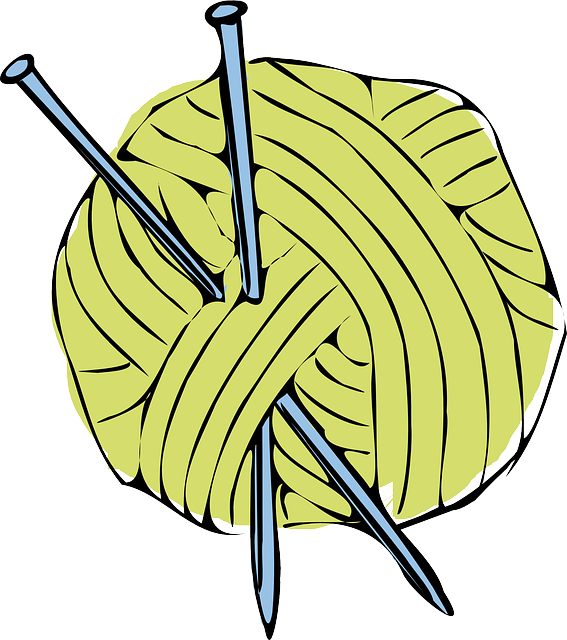
\includegraphics[height=0.2\textheight]{../img/ball_of_wool.png}
        \hspace*{4cm}
        
\includegraphics[height=0.2\textheight]{../img/ens.jpg}
   \end{center}
   \titlepage
}

% Proposition de plan :
% Introduction : présentation de l'équipe, 
% TriComp : Origine de l'idée, Compilateur ? Tricot ?
% Travail en amont : Problèmes à résoudre (allocation aiguilles, qqchose de général) -> "langage haut niveau"
% Coté logiciel : interface
% Difficultés rencontrées
% Améliorations possibles (complexifier fonctionnalites, reprendre les objectifs non traités du midterm)

\end{document}

